\documentclass{article}\usepackage[]{graphicx}\usepackage[]{xcolor}
% maxwidth is the original width if it is less than linewidth
% otherwise use linewidth (to make sure the graphics do not exceed the margin)
\makeatletter
\def\maxwidth{ %
  \ifdim\Gin@nat@width>\linewidth
    \linewidth
  \else
    \Gin@nat@width
  \fi
}
\makeatother

\definecolor{fgcolor}{rgb}{0.345, 0.345, 0.345}
\newcommand{\hlnum}[1]{\textcolor[rgb]{0.686,0.059,0.569}{#1}}%
\newcommand{\hlstr}[1]{\textcolor[rgb]{0.192,0.494,0.8}{#1}}%
\newcommand{\hlcom}[1]{\textcolor[rgb]{0.678,0.584,0.686}{\textit{#1}}}%
\newcommand{\hlopt}[1]{\textcolor[rgb]{0,0,0}{#1}}%
\newcommand{\hlstd}[1]{\textcolor[rgb]{0.345,0.345,0.345}{#1}}%
\newcommand{\hlkwa}[1]{\textcolor[rgb]{0.161,0.373,0.58}{\textbf{#1}}}%
\newcommand{\hlkwb}[1]{\textcolor[rgb]{0.69,0.353,0.396}{#1}}%
\newcommand{\hlkwc}[1]{\textcolor[rgb]{0.333,0.667,0.333}{#1}}%
\newcommand{\hlkwd}[1]{\textcolor[rgb]{0.737,0.353,0.396}{\textbf{#1}}}%
\let\hlipl\hlkwb

\usepackage{framed}
\makeatletter
\newenvironment{kframe}{%
 \def\at@end@of@kframe{}%
 \ifinner\ifhmode%
  \def\at@end@of@kframe{\end{minipage}}%
  \begin{minipage}{\columnwidth}%
 \fi\fi%
 \def\FrameCommand##1{\hskip\@totalleftmargin \hskip-\fboxsep
 \colorbox{shadecolor}{##1}\hskip-\fboxsep
     % There is no \\@totalrightmargin, so:
     \hskip-\linewidth \hskip-\@totalleftmargin \hskip\columnwidth}%
 \MakeFramed {\advance\hsize-\width
   \@totalleftmargin\z@ \linewidth\hsize
   \@setminipage}}%
 {\par\unskip\endMakeFramed%
 \at@end@of@kframe}
\makeatother

\definecolor{shadecolor}{rgb}{.97, .97, .97}
\definecolor{messagecolor}{rgb}{0, 0, 0}
\definecolor{warningcolor}{rgb}{1, 0, 1}
\definecolor{errorcolor}{rgb}{1, 0, 0}
\newenvironment{knitrout}{}{} % an empty environment to be redefined in TeX

\usepackage{alltt}
\usepackage[sc]{mathpazo}
\renewcommand{\sfdefault}{lmss}
\renewcommand{\ttdefault}{lmtt}
\usepackage[T1]{fontenc}
\usepackage{geometry}
\geometry{verbose,tmargin=2.5cm,bmargin=2.5cm,lmargin=2.5cm,rmargin=2.5cm}
\setcounter{secnumdepth}{2}
\setcounter{tocdepth}{2}
\usepackage[unicode=true,pdfusetitle,
 bookmarks=true,bookmarksnumbered=true,bookmarksopen=true,bookmarksopenlevel=2,
 breaklinks=false,pdfborder={0 0 1},backref=false,colorlinks=false]
 {hyperref}
\hypersetup{
 pdfstartview={XYZ null null 1}}

\makeatletter
%%%%%%%%%%%%%%%%%%%%%%%%%%%%%% User specified LaTeX commands.
\renewcommand{\textfraction}{0.05}
\renewcommand{\topfraction}{0.8}
\renewcommand{\bottomfraction}{0.8}
\renewcommand{\floatpagefraction}{0.75}

\makeatother
\IfFileExists{upquote.sty}{\usepackage{upquote}}{}
\begin{document}








The results below are generated from an R script.

\begin{knitrout}
\definecolor{shadecolor}{rgb}{0.969, 0.969, 0.969}\color{fgcolor}\begin{kframe}
\begin{alltt}
\hlcom{# Assignment: ASSIGNMENT 8_2}
\hlcom{# Name: Reppeto, Brian}
\hlcom{# Date: 2023-07-27}

\hlcom{## Load the ggplot2 package}

\hlkwd{library}\hlstd{(tidyverse)}
\hlkwd{library}\hlstd{(readxl)}
\hlkwd{library}\hlstd{(ggplot2)}
\hlkwd{library}\hlstd{(dplyr)}
\hlkwd{library}\hlstd{(conflicted)}
\hlkwd{library}\hlstd{(stats)}
\hlkwd{library}\hlstd{(car)}
\hlkwd{library}\hlstd{(lmtest)}
\hlkwd{library}\hlstd{(corrplot)}
\hlkwd{library}\hlstd{(lm.beta)}
\hlkwd{theme_set}\hlstd{(}\hlkwd{theme_minimal}\hlstd{())}

\hlcom{## Set the working directory to the root of your DSC 520 directory}
\hlkwd{setwd}\hlstd{(}\hlstr{"~/DSC520/Week 8"}\hlstd{)}

\hlcom{## Load the `data` to}
\hlstd{housing_df} \hlkwb{<-} \hlkwd{read_xlsx}\hlstd{(}\hlstr{"week-6-housing.xlsx"}\hlstd{)}


\hlcom{## 1.}
\hlstd{housing} \hlkwb{<-} \hlkwd{na.omit}\hlstd{(housing_df)}
\hlstd{housing} \hlkwb{<-}
  \hlkwd{rename}\hlstd{(housing_df,} \hlkwc{sale_price} \hlstd{= `Sale Price`,} \hlkwc{sale_date} \hlstd{= `Sale Date`)}

\hlstd{housing} \hlkwb{<-} \hlkwd{mutate}\hlstd{(housing,} \hlkwc{month} \hlstd{= lubridate} \hlopt{::} \hlkwd{month} \hlstd{(sale_date),}
                  \hlkwc{year} \hlstd{= lubridate} \hlopt{::} \hlkwd{year} \hlstd{(sale_date))}

\hlstd{housing} \hlkwb{<-} \hlkwd{mutate}\hlstd{(housing,} \hlkwc{sale_price_in_thous} \hlstd{= sale_price} \hlopt{/} \hlnum{1000}\hlstd{)}

\hlcom{# standardized the data to make easier to work with.}

\hlcom{## 2. Create two variables; one that will contain the variables Sale Price and }
\hlcom{## Square Foot of Lot (same variables used from previous assignment on simple }
\hlcom{## regression) and one that will contain Sale Price and several additional }
\hlcom{## predictors of your choice. Explain the basis for your additional predictor }
\hlcom{## selections.}

\hlstd{sale_price_sq_ft_df} \hlkwb{<-} \hlstd{housing [,}\hlkwd{c}\hlstd{(}\hlstr{"sale_price"}\hlstd{,}\hlstr{"sq_ft_lot"}\hlstd{)]}
\hlcom{#head(sale_price_sq_ft_df)}
\hlstd{housing_predictors_df} \hlkwb{<-}
  \hlstd{housing[,} \hlkwd{c}\hlstd{(}\hlstr{"sale_price"}\hlstd{,}\hlstr{"bedrooms"}\hlstd{,}
              \hlstr{"bath_full_count"}\hlstd{,}
              \hlstr{"year_built"}\hlstd{,}
              \hlstr{"square_feet_total_living"}\hlstd{,}\hlstr{"sale_date"}\hlstd{)]}
\hlkwd{head}\hlstd{(housing_predictors_df)}
\end{alltt}
\begin{verbatim}
## # A tibble: 6 x 6
##   sale_price bedrooms bath_full_count year_built square_feet_total_living
##        <dbl>    <dbl>           <dbl>      <dbl>                    <dbl>
## 1     698000        4               2       2003                     2810
## 2     649990        4               2       2006                     2880
## 3     572500        4               1       1987                     2770
## 4     420000        3               1       1968                     1620
## 5     369900        3               1       1980                     1440
## 6     184667        4               2       2005                     4160
## # i 1 more variable: sale_date <dttm>
\end{verbatim}
\begin{alltt}
\hlcom{## these items were chosen as they can help understand the pricing of the homes}



\hlcom{## 3. Execute a summary() function on two variables defined in the previous }
\hlcom{## step to compare the model results. What are the R2 and Adjusted R2 }
\hlcom{## statistics? Explain what these results tell you about the overall model. }
\hlcom{## Did the inclusion of the additional predictors help explain any large }
\hlcom{## variations found in Sale Price?}


\hlstd{model_1} \hlkwb{<-} \hlkwd{lm}\hlstd{(sale_price} \hlopt{~} \hlstd{sq_ft_lot,} \hlkwc{data} \hlstd{= sale_price_sq_ft_df)}
\hlkwd{summary}\hlstd{(model_1)}
\end{alltt}
\begin{verbatim}
## 
## Call:
## lm(formula = sale_price ~ sq_ft_lot, data = sale_price_sq_ft_df)
## 
## Residuals:
##      Min       1Q   Median       3Q      Max 
## -2016064  -194842   -63293    91565  3735109 
## 
## Coefficients:
##              Estimate Std. Error t value Pr(>|t|)    
## (Intercept) 6.418e+05  3.800e+03  168.90   <2e-16 ***
## sq_ft_lot   8.510e-01  6.217e-02   13.69   <2e-16 ***
## ---
## Signif. codes:  0 '***' 0.001 '**' 0.01 '*' 0.05 '.' 0.1 ' ' 1
## 
## Residual standard error: 401500 on 12863 degrees of freedom
## Multiple R-squared:  0.01435,	Adjusted R-squared:  0.01428 
## F-statistic: 187.3 on 1 and 12863 DF,  p-value: < 2.2e-16
\end{verbatim}
\begin{alltt}
\hlstd{model_2} \hlkwb{<-}
  \hlkwd{lm}\hlstd{(}
    \hlstd{sale_price} \hlopt{~} \hlstd{bedrooms} \hlopt{+} \hlstd{bath_full_count} \hlopt{+} \hlstd{year_built} \hlopt{+}
    \hlstd{square_feet_total_living} \hlopt{+} \hlstd{sale_date,}
    \hlkwc{data} \hlstd{= housing_predictors_df}
  \hlstd{)}
\hlkwd{summary}\hlstd{(model_2)}
\end{alltt}
\begin{verbatim}
## 
## Call:
## lm(formula = sale_price ~ bedrooms + bath_full_count + year_built + 
##     square_feet_total_living + sale_date, data = housing_predictors_df)
## 
## Residuals:
##      Min       1Q   Median       3Q      Max 
## -1726837  -120499   -38306    45397  3914306 
## 
## Coefficients:
##                            Estimate Std. Error t value Pr(>|t|)    
## (Intercept)              -4.705e+06  4.210e+05 -11.175  < 2e-16 ***
## bedrooms                 -1.491e+04  4.514e+03  -3.304 0.000956 ***
## bath_full_count           1.826e+04  6.087e+03   3.000 0.002703 ** 
## year_built                2.351e+03  2.114e+02  11.121  < 2e-16 ***
## square_feet_total_living  1.740e+02  4.416e+00  39.396  < 2e-16 ***
## sale_date                 1.959e-04  3.043e-05   6.439 1.25e-10 ***
## ---
## Signif. codes:  0 '***' 0.001 '**' 0.01 '*' 0.05 '.' 0.1 ' ' 1
## 
## Residual standard error: 356800 on 12859 degrees of freedom
## Multiple R-squared:  0.2219,	Adjusted R-squared:  0.2216 
## F-statistic: 733.5 on 5 and 12859 DF,  p-value: < 2.2e-16
\end{verbatim}
\begin{alltt}
\hlcom{# Since model_2 has a higher r2 of 0.2219 than model_1 of 0.01435, I can}
\hlcom{# conclude that the additional predictors did help.}


\hlcom{## 4. Considering the parameters of the multiple regression model you have }
\hlcom{## created. What are the standardized betas for each parameter and what do the }
\hlcom{## values indicate?}



\hlstd{standardized_betas_model_1} \hlkwb{<-} \hlkwd{lm.beta}\hlstd{(model_1)}
\hlkwd{print}\hlstd{(standardized_betas_model_1)}
\end{alltt}
\begin{verbatim}
## 
## Call:
## lm(formula = sale_price ~ sq_ft_lot, data = sale_price_sq_ft_df)
## 
## Standardized Coefficients::
## (Intercept)   sq_ft_lot 
##          NA   0.1198122
\end{verbatim}
\begin{alltt}
\hlcom{# A positive value for sq_ft_lot indicates that an increase in the standard}
\hlcom{# deviation of sq_ft_lot is associated with an increase in the stnd. deviation}
\hlcom{# of sale_price}
\hlstd{standardized_betas_model_2} \hlkwb{<-} \hlkwd{lm.beta}\hlstd{(model_2)}
\hlkwd{print}\hlstd{(standardized_betas_model_2)}
\end{alltt}
\begin{verbatim}
## 
## Call:
## lm(formula = sale_price ~ bedrooms + bath_full_count + year_built + 
##     square_feet_total_living + sale_date, data = housing_predictors_df)
## 
## Standardized Coefficients::
##              (Intercept)                 bedrooms          bath_full_count 
##                       NA              -0.03231038               0.02939034 
##               year_built square_feet_total_living                sale_date 
##               0.10012380               0.42583932               0.05017694
\end{verbatim}
\begin{alltt}
\hlcom{# A positive value for the other parameters indicates that an increase in the }
\hlcom{# standard deviation of the other parameters is associated with an increase }
\hlcom{# in the standard deviation of sale_price.  A negative number indicates the }
\hlcom{# a possible inverse relationship with sale_price.}

\hlcom{## 5. Calculate the confidence intervals for the parameters in your model and }
\hlcom{## explain what the results indicate.}


\hlstd{conf_intervals_model_1} \hlkwb{<-} \hlkwd{confint}\hlstd{(model_1)}

\hlstd{conf_intervals_model_2} \hlkwb{<-} \hlkwd{confint}\hlstd{(model_2)}

\hlkwd{print}\hlstd{(conf_intervals_model_1)}
\end{alltt}
\begin{verbatim}
##                    2.5 %       97.5 %
## (Intercept) 6.343730e+05 6.492698e+05
## sq_ft_lot   7.291208e-01 9.728641e-01
\end{verbatim}
\begin{alltt}
\hlkwd{print}\hlstd{(conf_intervals_model_2)}
\end{alltt}
\begin{verbatim}
##                                  2.5 %        97.5 %
## (Intercept)              -5.530304e+06 -3.879729e+06
## bedrooms                 -2.376055e+04 -6.065495e+03
## bath_full_count           6.330974e+03  3.019318e+04
## year_built                1.936801e+03  2.765612e+03
## square_feet_total_living  1.653168e+02  1.826288e+02
## sale_date                 1.362791e-04  2.555637e-04
\end{verbatim}
\begin{alltt}
\hlcom{# Based on the results, we can conclude that there is a 97.5% confidence that }
\hlcom{# the true population value of the parameter lies somewhere between the %'s.}
\hlcom{# Since the interval does not include zero, we can conclude that the parameter }
\hlcom{# is statistically significant.}

\hlcom{## 6. Assess the improvement of the new model compared to your original model }
\hlcom{## (simple regression model) by testing whether this change is significant by }
\hlcom{## performing an analysis of variance.}

\hlstd{anova_result} \hlkwb{<-} \hlkwd{anova}\hlstd{(model_1, model_2)}
\hlkwd{print}\hlstd{(anova_result)}
\end{alltt}
\begin{verbatim}
## Analysis of Variance Table
## 
## Model 1: sale_price ~ sq_ft_lot
## Model 2: sale_price ~ bedrooms + bath_full_count + year_built + square_feet_total_living + 
##     sale_date
##   Res.Df        RSS Df  Sum of Sq      F    Pr(>F)    
## 1  12863 2.0734e+15                                   
## 2  12859 1.6368e+15  4 4.3661e+14 857.55 < 2.2e-16 ***
## ---
## Signif. codes:  0 '***' 0.001 '**' 0.01 '*' 0.05 '.' 0.1 ' ' 1
\end{verbatim}
\begin{alltt}
\hlcom{## 7. Perform casewise diagnostics to identify outliers and/or influential }
\hlcom{## cases, storing each function's output in a dataframe assigned to a unique }
\hlcom{## variable name.}

\hlstd{housing}\hlopt{$}\hlstd{residuals_mod1} \hlkwb{<-} \hlkwd{resid}\hlstd{(model_1)}
\hlstd{housing}\hlopt{$}\hlstd{studentized.residuals_mod1} \hlkwb{<-} \hlkwd{rstudent}\hlstd{(model_1)}
\hlstd{housing}\hlopt{$}\hlstd{standardized.residuals_mod1} \hlkwb{<-} \hlkwd{rstandard}\hlstd{(model_1)}

\hlstd{housing}\hlopt{$}\hlstd{residuals_mod2} \hlkwb{<-} \hlkwd{resid}\hlstd{(model_2)}
\hlstd{housing}\hlopt{$}\hlstd{studentized.residuals_mod2} \hlkwb{<-} \hlkwd{rstudent}\hlstd{(model_2)}
\hlstd{housing}\hlopt{$}\hlstd{standardized.residuals_mod2} \hlkwb{<-} \hlkwd{rstandard}\hlstd{(model_2)}
\hlcom{## Influential cases}
\hlstd{housing}\hlopt{$}\hlstd{dffit_mod1} \hlkwb{<-} \hlkwd{dffits}\hlstd{(model_1)}
\hlstd{housing}\hlopt{$}\hlstd{leverage_mod1} \hlkwb{<-} \hlkwd{hatvalues}\hlstd{(model_1)}
\hlstd{housing}\hlopt{$}\hlstd{covariance.ratios_mod1} \hlkwb{<-} \hlkwd{covratio}\hlstd{(model_1)}
\hlstd{housing}\hlopt{$}\hlstd{cooks.distance_mod1} \hlkwb{<-} \hlkwd{cooks.distance}\hlstd{(model_1)}
\hlstd{housing}\hlopt{$}\hlstd{dfbeta_mod2} \hlkwb{<-} \hlkwd{dfbeta}\hlstd{(model_1)}
\hlstd{housing}\hlopt{$}\hlstd{dffit_mod1} \hlkwb{<-} \hlkwd{dffits}\hlstd{(model_1)}

\hlstd{housing}\hlopt{$}\hlstd{leverage_mod2} \hlkwb{<-} \hlkwd{hatvalues}\hlstd{(model_2)}
\hlstd{housing}\hlopt{$}\hlstd{covariance.ratios_mod2} \hlkwb{<-} \hlkwd{covratio}\hlstd{(model_2)}
\hlstd{housing}\hlopt{$}\hlstd{cooks.distance_mod2} \hlkwb{<-} \hlkwd{cooks.distance}\hlstd{(model_2)}
\hlstd{housing}\hlopt{$}\hlstd{dfbeta_mod2} \hlkwb{<-} \hlkwd{dfbeta}\hlstd{(model_2)}
\hlkwd{summary}\hlstd{(housing)}
\end{alltt}
\begin{verbatim}
##    sale_date                        sale_price       sale_reason    sale_instrument 
##  Min.   :2006-01-03 00:00:00.00   Min.   :    698   Min.   : 0.00   Min.   : 0.000  
##  1st Qu.:2008-07-07 00:00:00.00   1st Qu.: 460000   1st Qu.: 1.00   1st Qu.: 3.000  
##  Median :2011-11-17 00:00:00.00   Median : 593000   Median : 1.00   Median : 3.000  
##  Mean   :2011-07-28 15:07:32.48   Mean   : 660738   Mean   : 1.55   Mean   : 3.678  
##  3rd Qu.:2014-06-05 00:00:00.00   3rd Qu.: 750000   3rd Qu.: 1.00   3rd Qu.: 3.000  
##  Max.   :2016-12-16 00:00:00.00   Max.   :4400000   Max.   :19.00   Max.   :27.000  
##  sale_warning         sitetype          addr_full              zip5      
##  Length:12865       Length:12865       Length:12865       Min.   :98052  
##  Class :character   Class :character   Class :character   1st Qu.:98052  
##  Mode  :character   Mode  :character   Mode  :character   Median :98052  
##                                                           Mean   :98053  
##                                                           3rd Qu.:98053  
##                                                           Max.   :98074  
##    ctyname           postalctyn             lon              lat        building_grade 
##  Length:12865       Length:12865       Min.   :-122.2   Min.   :47.46   Min.   : 2.00  
##  Class :character   Class :character   1st Qu.:-122.1   1st Qu.:47.67   1st Qu.: 8.00  
##  Mode  :character   Mode  :character   Median :-122.1   Median :47.69   Median : 8.00  
##                                        Mean   :-122.1   Mean   :47.68   Mean   : 8.24  
##                                        3rd Qu.:-122.0   3rd Qu.:47.70   3rd Qu.: 9.00  
##                                        Max.   :-121.9   Max.   :47.73   Max.   :13.00  
##  square_feet_total_living    bedrooms      bath_full_count  bath_half_count 
##  Min.   :  240            Min.   : 0.000   Min.   : 0.000   Min.   :0.0000  
##  1st Qu.: 1820            1st Qu.: 3.000   1st Qu.: 1.000   1st Qu.:0.0000  
##  Median : 2420            Median : 4.000   Median : 2.000   Median :1.0000  
##  Mean   : 2540            Mean   : 3.479   Mean   : 1.798   Mean   :0.6134  
##  3rd Qu.: 3110            3rd Qu.: 4.000   3rd Qu.: 2.000   3rd Qu.:1.0000  
##  Max.   :13540            Max.   :11.000   Max.   :23.000   Max.   :8.0000  
##  bath_3qtr_count   year_built   year_renovated    current_zoning       sq_ft_lot      
##  Min.   :0.000   Min.   :1900   Min.   :   0.00   Length:12865       Min.   :    785  
##  1st Qu.:0.000   1st Qu.:1979   1st Qu.:   0.00   Class :character   1st Qu.:   5355  
##  Median :0.000   Median :1998   Median :   0.00   Mode  :character   Median :   7965  
##  Mean   :0.494   Mean   :1993   Mean   :  26.24                      Mean   :  22229  
##  3rd Qu.:1.000   3rd Qu.:2007   3rd Qu.:   0.00                      3rd Qu.:  12632  
##  Max.   :8.000   Max.   :2016   Max.   :2016.00                      Max.   :1631322  
##   prop_type          present_use          month             year      sale_price_in_thous
##  Length:12865       Min.   :  0.000   Min.   : 1.000   Min.   :2006   Min.   :   0.698   
##  Class :character   1st Qu.:  2.000   1st Qu.: 4.000   1st Qu.:2008   1st Qu.: 460.000   
##  Mode  :character   Median :  2.000   Median : 7.000   Median :2011   Median : 593.000   
##                     Mean   :  6.598   Mean   : 6.772   Mean   :2011   Mean   : 660.738   
##                     3rd Qu.:  2.000   3rd Qu.: 9.000   3rd Qu.:2014   3rd Qu.: 750.000   
##                     Max.   :300.000   Max.   :12.000   Max.   :2016   Max.   :4400.000   
##  residuals_mod1     studentized.residuals_mod1 standardized.residuals_mod1
##  Min.   :-2016064   Min.   :-5.190538          Min.   :-5.185311          
##  1st Qu.: -194842   1st Qu.:-0.485311          1st Qu.:-0.485326          
##  Median :  -63293   Median :-0.157650          Median :-0.157656          
##  Mean   :       0   Mean   : 0.000161          Mean   :-0.000013          
##  3rd Qu.:   91565   3rd Qu.: 0.228068          3rd Qu.: 0.228076          
##  Max.   : 3735109   Max.   : 9.334760          Max.   : 9.303661          
##  residuals_mod2     studentized.residuals_mod2 standardized.residuals_mod2
##  Min.   :-1726837   Min.   :-4.855550          Min.   :-4.851293          
##  1st Qu.: -120499   1st Qu.:-0.337792          1st Qu.:-0.337804          
##  Median :  -38306   Median :-0.107374          Median :-0.107379          
##  Mean   :       0   Mean   : 0.000215          Mean   :-0.000008          
##  3rd Qu.:   45397   3rd Qu.: 0.127256          3rd Qu.: 0.127260          
##  Max.   : 3914306   Max.   :11.029385          Max.   :10.978006          
##    dffit_mod1         leverage_mod1       covariance.ratios_mod1 cooks.distance_mod1
##  Min.   :-1.3364399   Min.   :7.773e-05   Min.   :0.9868         Min.   :0.0000000  
##  1st Qu.:-0.0044992   1st Qu.:8.177e-05   1st Qu.:1.0002         1st Qu.:0.0000015  
##  Median :-0.0014833   Median :8.355e-05   Median :1.0002         Median :0.0000062  
##  Mean   :-0.0001268   Mean   :1.555e-04   Mean   :1.0002         Mean   :0.0003245  
##  3rd Qu.: 0.0021122   3rd Qu.:8.539e-05   3rd Qu.:1.0002         3rd Qu.:0.0000182  
##  Max.   : 1.3832441   Max.   :6.217e-02   Max.   :1.0620         Max.   :0.9534315  
##  dfbeta_mod2.(Intercept)   dfbeta_mod2.bedrooms    dfbeta_mod2.bath_full_count  dfbeta_mod2.year_built   dfbeta_mod2.square_feet_total_living   dfbeta_mod2.sale_date 
##  Min.   :-199853.91       Min.   :-1076.1703       Min.   :-8240.248        Min.   :-70.62678        Min.   :-1.7986286       Min.   :-2.267598e-06                   
##  1st Qu.:   -317.16       1st Qu.:   -5.3956       1st Qu.:   -6.831        1st Qu.: -0.37515        1st Qu.:-0.0030897       1st Qu.:-4.082600e-08                   
##  Median :     73.63       Median :   -0.0763       Median :   -0.103        Median : -0.03840        Median : 0.0003065       Median : 4.430000e-10                   
##  Mean   :     -1.67       Mean   :    0.0056       Mean   :   -0.073        Mean   :  0.00087        Mean   : 0.0000137       Mean   : 9.000000e-12                   
##  3rd Qu.:    742.94       3rd Qu.:    5.3046       3rd Qu.:    6.103        3rd Qu.:  0.15877        3rd Qu.: 0.0053540       3rd Qu.: 4.383000e-08                   
##  Max.   : 143261.02       Max.   :  774.4194       Max.   : 1354.434        Max.   :103.88819        Max.   : 1.6924877       Max.   : 4.168366e-06                   
##  leverage_mod2       covariance.ratios_mod2 cooks.distance_mod2
##  Min.   :0.0001082   Min.   :0.9466         Min.   :0.000e+00  
##  1st Qu.:0.0002690   1st Qu.:1.0007         1st Qu.:8.100e-07  
##  Median :0.0003778   Median :1.0008         Median :3.690e-06  
##  Mean   :0.0004664   Mean   :1.0005         Mean   :1.262e-04  
##  3rd Qu.:0.0005169   3rd Qu.:1.0009         3rd Qu.:1.171e-05  
##  Max.   :0.1202763   Max.   :1.1301         Max.   :3.077e-01
\end{verbatim}
\begin{alltt}
\hlcom{## 8. Calculate the standardized residuals using the appropriate command, }
\hlcom{## specifying those that are +-2, storing the results of large residuals in }
\hlcom{## a variable you create.}

\hlstd{standardized_residuals} \hlkwb{<-} \hlkwd{rstandard}\hlstd{(model_2)}

\hlstd{large_residuals} \hlkwb{<-} \hlkwd{abs}\hlstd{(standardized_residuals)} \hlopt{>=} \hlnum{2}

\hlstd{data_points_with_large_residuals} \hlkwb{<-} \hlstd{housing_predictors_df[large_residuals, ]}

\hlkwd{print}\hlstd{(data_points_with_large_residuals)}
\end{alltt}
\begin{verbatim}
## # A tibble: 328 x 6
##    sale_price bedrooms bath_full_count year_built square_feet_total_living
##         <dbl>    <dbl>           <dbl>      <dbl>                    <dbl>
##  1     184667        4               2       2005                     4160
##  2     265000        4               4       2007                     4920
##  3    1390000        0               1       1955                      660
##  4     390000        5               4       2008                     5800
##  5    1588359        2               2       2005                     3360
##  6    1450000        2               1       1918                      900
##  7     163000        4               2       2014                     4710
##  8     270000        4              23       2016                     5060
##  9     200000        5               1       2008                     6880
## 10     187000        4               2       2008                     5140
## # i 318 more rows
## # i 1 more variable: sale_date <dttm>
\end{verbatim}
\begin{alltt}
\hlcom{## 9. Use the appropriate function to show the sum of large residuals.}

\hlstd{sum_large_residuals} \hlkwb{<-} \hlkwd{sum}\hlstd{(large_residuals)}
\hlkwd{print}\hlstd{(sum_large_residuals)}
\end{alltt}
\begin{verbatim}
## [1] 328
\end{verbatim}
\begin{alltt}
\hlcom{## 10. Which specific variables have large residuals (only cases that evaluate }
\hlcom{## as TRUE)?}
\hlkwd{print}\hlstd{(data_points_with_large_residuals[,} \hlkwd{c}\hlstd{(}
  \hlstr{"bedrooms"}\hlstd{,}
  \hlstr{"bath_full_count"}\hlstd{,}
  \hlstr{"year_built"}\hlstd{,}
  \hlstr{"square_feet_total_living"}\hlstd{,}
  \hlstr{"sale_date"}
\hlstd{)])}
\end{alltt}
\begin{verbatim}
## # A tibble: 328 x 5
##    bedrooms bath_full_count year_built square_feet_total_living sale_date          
##       <dbl>           <dbl>      <dbl>                    <dbl> <dttm>             
##  1        4               2       2005                     4160 2006-01-03 00:00:00
##  2        4               4       2007                     4920 2006-01-11 00:00:00
##  3        0               1       1955                      660 2006-02-15 00:00:00
##  4        5               4       2008                     5800 2006-03-03 00:00:00
##  5        2               2       2005                     3360 2006-03-20 00:00:00
##  6        2               1       1918                      900 2006-03-21 00:00:00
##  7        4               2       2014                     4710 2006-03-27 00:00:00
##  8        4              23       2016                     5060 2006-03-28 00:00:00
##  9        5               1       2008                     6880 2006-03-29 00:00:00
## 10        4               2       2008                     5140 2006-04-10 00:00:00
## # i 318 more rows
\end{verbatim}
\begin{alltt}
\hlcom{## 11. Investigate further by calculating the leverage, cooks distance, and }
\hlcom{## covariance rations. Comment on all cases that are problematics.}
\hlcom{# Load necessary libraries (if not already loaded)}



\hlstd{leverage} \hlkwb{<-} \hlkwd{hatvalues}\hlstd{(model_2)}


\hlstd{cooks_distance} \hlkwb{<-} \hlkwd{cooks.distance}\hlstd{(model_2)}


\hlstd{cov_ratios} \hlkwb{<-} \hlkwd{covratio}\hlstd{(model_2)}


\hlstd{diagnostics_df} \hlkwb{<-} \hlkwd{data.frame}\hlstd{(}\hlkwc{Leverage} \hlstd{= leverage,}
                             \hlkwc{Cooks_Distance} \hlstd{= cooks_distance,}
                             \hlkwc{covariance_ratio} \hlstd{= cov_ratios)}

\hlkwd{print}\hlstd{(diagnostics_df)}
\end{alltt}
\begin{verbatim}
##         Leverage Cooks_Distance covariance_ratio
## 1   0.0003684559   1.305166e-08        1.0008354
## 2   0.0003868911   1.951519e-06        1.0008398
## 3   0.0005514774   2.386793e-06        1.0010066
## 4   0.0005085812   2.631430e-07        1.0009744
## 5   0.0004450780   4.293670e-07        1.0009095
## 6   0.0005777317   4.234018e-04        0.9989941
## 7   0.0007459010   3.073992e-05        1.0010981
## 8   0.0004674794   2.142551e-06        1.0009218
## 9   0.0007309459   4.182838e-05        1.0010383
## 10  0.0005620735   1.671221e-06        1.0010211
## 11  0.0003637092   6.556351e-07        1.0008257
## 12  0.0003547655   7.644224e-06        1.0007614
## 13  0.0005318602   9.970487e-07        1.0009939
## 14  0.0004688041   9.563597e-05        1.0003647
## 15  0.0004625362   2.288947e-06        1.0009158
## 16  0.0003545507   1.005118e-05        1.0007422
## 17  0.0005247549   1.340106e-05        1.0009205
## 18  0.0004056907   2.305340e-06        1.0008569
## 19  0.0005983385   5.353191e-06        1.0010406
## 20  0.0004398576   1.378094e-06        1.0008982
## 21  0.0005611711   2.745284e-06        1.0010148
## 22  0.0003453218   9.850090e-06        1.0007324
## 23  0.0007100147   9.592994e-07        1.0011738
## 24  0.0005669091   5.818085e-06        1.0010055
## 25  0.0014021969   1.302076e-03        0.9992734
## 26  0.0006090327   2.249127e-04        1.0000425
## 27  0.0004161989   1.166293e-06        1.0008754
## 28  0.0003816868   1.332758e-07        1.0008478
## 29  0.0003715626   7.309546e-06        1.0007835
## 30  0.0005695436   3.631387e-08        1.0010367
## 31  0.0006107318   4.336954e-06        1.0010582
## 32  0.0004845094   9.374376e-06        1.0008975
## 33  0.0004180954   3.368790e-06        1.0008626
## 34  0.0007001643   4.456109e-06        1.0011499
## 35  0.0003899026   5.129561e-06        1.0008201
## 36  0.0003624638   7.278718e-06        1.0007732
## 37  0.0005687266   1.352232e-08        1.0010360
## 38  0.0003619829   1.917648e-06        1.0008142
## 39  0.0003632495   1.091127e-06        1.0008219
## 40  0.0003923748   4.077726e-07        1.0008565
## 41  0.0009100902   6.257405e-05        1.0011855
## 42  0.0005051812   6.644086e-06        1.0009356
## 43  0.0004302987   2.404455e-06        1.0008818
## 44  0.0005781387   1.875112e-06        1.0010364
## 45  0.0004950999   4.572508e-07        1.0009597
## 46  0.0006575777   2.527438e-08        1.0011249
## 47  0.0013328434   1.619985e-04        1.0014616
## 48  0.0004808132   3.293352e-06        1.0009288
## 49  0.0004211203   2.370705e-06        1.0008725
## 50  0.0006126475   1.698880e-05        1.0010024
## 51  0.0005555801   5.644098e-07        1.0010200
## 52  0.0003744423   3.089623e-09        1.0008415
## 53  0.0003508836   2.109389e-07        1.0008162
## 54  0.0004073869   1.870764e-06        1.0008616
## 55  0.0005727492   6.909632e-07        1.0010367
## 56  0.0006605613   1.229182e-07        1.0011275
## 57  0.0005864692   1.089170e-06        1.0010486
## 58  0.0004220959   1.743814e-07        1.0008880
## 59  0.0004615350   6.981297e-07        1.0009245
## 60  0.0006458151   1.028638e-04        1.0006672
## 61  0.0005713908   2.177277e-07        1.0010376
## 62  0.0004603859   7.047150e-06        1.0008847
## 63  0.0007754329   4.648694e-07        1.0012414
## 64  0.0003803739   1.288030e-07        1.0008465
## 65  0.0010131760   3.928277e-06        1.0014705
## 66  0.0006494240   1.248623e-06        1.0011115
## 67  0.0004459774   9.785271e-06        1.0008517
## 68  0.0005581077   9.804475e-07        1.0010205
## 69  0.0003817146   3.723761e-06        1.0008214
## 70  0.0003492163   6.054898e-06        1.0007677
## 71  0.0003808767   8.271228e-05        1.0002398
## 72  0.0023187577   9.494643e-04        1.0016456
## 73  0.0003620302   6.995575e-05        1.0002880
## 74  0.0005878170   2.154599e-06        1.0010449
## 75  0.0004604567   5.764895e-06        1.0008925
## 76  0.0004868165   3.574156e-06        1.0009334
## 77  0.0003560126   1.611617e-06        1.0008104
## 78  0.0005700560   1.865293e-08        1.0010373
## 79  0.0005983060   1.314327e-05        1.0010041
## 80  0.0005604775   1.286966e-06        1.0010213
## 81  0.0006557836   1.718106e-05        1.0010499
## 82  0.0003543032   3.255539e-07        1.0008187
## 83  0.0005687879   1.139350e-06        1.0010305
## 84  0.0003721056   3.624393e-06        1.0008119
## 85  0.0003971228   4.593634e-06        1.0008318
## 86  0.0003718705   1.662892e-06        1.0008264
## 87  0.0013965587   1.335038e-05        1.0018391
## 88  0.0005062635   1.173896e-07        1.0009728
## 89  0.0005244332   3.968528e-07        1.0009896
## 90  0.0003695637   1.254909e-05        1.0007415
## 91  0.0004773800   1.822560e-06        1.0009339
## 92  0.0015453410   3.372677e-04        1.0014040
## 93  0.0003621435   2.524607e-07        1.0008272
## 94  0.0003437795   6.001293e-06        1.0007619
## 95  0.0004988017   1.371677e-06        1.0009583
## 96  0.0005912224   5.845986e-08        1.0010583
## 97  0.0003774199   5.899512e-06        1.0008007
## 98  0.0007159351   3.148725e-05        1.0010603
## 99  0.0004128218   1.746495e-06        1.0008681
## 100 0.0005015752   2.341099e-07        1.0009675
## 101 0.0005590609   1.855461e-06        1.0010171
## 102 0.0006676855   6.524859e-09        1.0011351
## 103 0.0004149160   6.056326e-06        1.0008411
## 104 0.0006955807   1.819494e-05        1.0010899
## 105 0.0006955807   1.819494e-05        1.0010899
## 106 0.0004809433   3.504408e-06        1.0009277
## 107 0.0004558644   1.184123e-07        1.0009223
## 108 0.0014739248   8.001921e-04        1.0004239
## 109 0.0003685189   2.744859e-09        1.0008355
## 110 0.0006984992   3.136825e-06        1.0011535
## 111 0.0005586874   1.824822e-06        1.0010168
## 112 0.0005297748   5.315816e-07        1.0009942
## 113 0.0003447376   5.335387e-06        1.0007684
## 114 0.0005474665   1.704430e-06        1.0010060
## 115 0.0020210388   3.465134e-03        0.9977001
## 116 0.0004408038   2.127424e-04        0.9995569
## 117 0.0005663560   3.435227e-06        1.0010167
## 118 0.0005850010   1.398610e-07        1.0010517
## 119 0.0006096217   1.668039e-06        1.0010693
## 120 0.0005362770   3.212440e-06        1.0009868
## 121 0.0005223600   2.734594e-07        1.0009881
## 122 0.0003748265   3.781092e-08        1.0008416
## 123 0.0003692546   2.753435e-06        1.0008154
## 124 0.0005733574   8.080432e-06        1.0010012
## 125 0.0004411921   1.019658e-07        1.0009077
## 126 0.0015376936   2.217426e-09        1.0020075
## 127 0.0005679838   4.475266e-06        1.0010132
## 128 0.0006196773   8.643791e-07        1.0010832
## 129 0.0005535659   9.826938e-06        1.0009711
## 130 0.0003682756   8.702815e-07        1.0008287
## 131 0.0004938587   3.273706e-05        1.0007754
## 132 0.0005212289   5.267588e-07        1.0009856
## 133 0.0005148625   2.129064e-06        1.0009705
## 134 0.0005748021   6.197237e-07        1.0010391
## 135 0.0006041514   6.527632e-06        1.0010413
## 136 0.0007069288   1.874634e-08        1.0011744
## 137 0.0004450669   2.042331e-10        1.0009122
## 138 0.0006183190   7.737316e-06        1.0010507
## 139 0.0003751795   7.424613e-07        1.0008367
## 140 0.0004303112   3.338374e-06        1.0008757
## 141 0.0005115878   1.891795e-07        1.0009778
## 142 0.0003629172   2.549574e-06        1.0008103
## 143 0.0005388058   2.428949e-07        1.0010048
## 144 0.0005218376   2.459401e-07        1.0009878
## 145 0.0013659414   5.471111e-06        1.0018240
## 146 0.0003469759   3.414972e-06        1.0007864
## 147 0.0003556538   6.935226e-07        1.0008172
## 148 0.0005680913   1.779151e-06        1.0010266
## 149 0.0004274486   1.222438e-07        1.0008938
## 150 0.0005199478   2.401449e-06        1.0009743
## 151 0.0003439498   5.057332e-06        1.0007698
## 152 0.0005610522   1.761463e-07        1.0010275
## 153 0.0003554453   6.937242e-07        1.0008170
## 154 0.0003438172   9.593522e-06        1.0007327
## 155 0.0004274092   1.055308e-06        1.0008876
## 156 0.0005199425   1.869820e-06        1.0009771
## 157 0.0005093878   6.933031e-09        1.0009766
## 158 0.0004976797   1.159476e-08        1.0009648
## 159 0.0004255691   3.215104e-06        1.0008715
## 160 0.0042697900   2.598287e-03        1.0030536
## 161 0.0011933425   1.003390e-05        1.0016385
## 162 0.0004045224   3.079784e-06        1.0008503
## 163 0.0005638067   2.295838e-07        1.0010300
## 164 0.0006758798   1.727348e-06        1.0011362
## 165 0.0003938454   1.965680e-06        1.0008469
## 166 0.0003881512   1.529355e-06        1.0008442
## 167 0.0003429046   6.541037e-06        1.0007565
## 168 0.0004313511   7.726936e-07        1.0008934
## 169 0.0005606138   1.299241e-06        1.0010214
## 170 0.0005081559   3.685363e-06        1.0009551
## 171 0.0004610691   5.478182e-08        1.0009279
## 172 0.0005958180   2.581904e-04        0.9998501
## 173 0.0003254381   6.640586e-07        1.0007867
## 174 0.0003297348   1.733180e-07        1.0007953
## 175 0.0004302824   3.570609e-06        1.0008742
## 176 0.0004088441   1.405055e-06        1.0008663
## 177 0.0009016030   4.800074e-06        1.0013547
## 178 0.0015205592   1.467936e-03        0.9992894
## 179 0.0003597348   1.916857e-07        1.0008253
## 180 0.0003591319   3.757766e-07        1.0008232
## 181 0.0003772137   2.173059e-09        1.0008442
## 182 0.0005183802   4.607296e-06        1.0009607
## 183 0.0005756999   2.087063e-09        1.0010430
## 184 0.0007631328   1.796600e-05        1.0011649
## 185 0.0004720669   2.218975e-06        1.0009261
## 186 0.0003935946   2.326090e-06        1.0008441
## 187 0.0004645734   1.386351e-06        1.0009234
## 188 0.0005908248   1.786202e-07        1.0010573
## 189 0.0004427390   1.284861e-07        1.0009091
## 190 0.0004189699   2.117616e-05        1.0007445
## 191 0.0003660184   1.841408e-05        1.0006921
## 192 0.0006398299   2.300110e-06        1.0010972
## 193 0.0003980171   1.812038e-07        1.0008638
## 194 0.0005536466   1.084213e-05        1.0009661
## 195 0.0005998932   3.812837e-06        1.0010495
## 196 0.0016411530   9.725211e-05        1.0019454
## 197 0.0003500445   2.769230e-06        1.0007949
## 198 0.0004168280   1.119713e-07        1.0008832
## 199 0.0003574373   7.563158e-11        1.0008245
## 200 0.0003597998   3.945031e-06        1.0007961
## 201 0.0004556501   5.820964e-07        1.0009192
## 202 0.0004009913   4.466129e-06        1.0008369
## 203 0.0004785687   1.127358e-07        1.0009451
## 204 0.0005582643   7.473593e-07        1.0010218
## 205 0.0007559896   8.503001e-06        1.0011921
## 206 0.0004073984   3.242260e-06        1.0008522
## 207 0.0005385779   1.346595e-05        1.0009358
## 208 0.0006169499   5.718687e-05        1.0008247
## 209 0.0003694554   1.769773e-06        1.0008231
## 210 0.0004281306   2.640441e-07        1.0008935
## 211 0.0031709326   7.757949e-06        1.0036424
## 212 0.0004297449   4.172060e-07        1.0008941
## 213 0.0004932960   6.511374e-08        1.0009601
## 214 0.0008267757   1.537854e-04        1.0007737
## 215 0.0004080319   1.180241e-05        1.0007941
## 216 0.0009918220   5.140873e-06        1.0014455
## 217 0.0003671618   7.714686e-07        1.0008283
## 218 0.0006966032   1.109460e-06        1.0011597
## 219 0.0005444397   9.238269e-07        1.0010070
## 220 0.0005933799   4.066071e-08        1.0010605
## 221 0.0004195322   7.182745e-08        1.0008862
## 222 0.0006583440   3.694826e-04        0.9995549
## 223 0.0007079928   2.020697e-08        1.0011755
## 224 0.0003277005   5.125628e-09        1.0007946
## 225 0.0004703493   2.896804e-07        1.0009358
## 226 0.0006767348   2.141867e-06        1.0011354
## 227 0.0005438580   1.348866e-06        1.0010042
## 228 0.0008787460   6.065176e-06        1.0013273
## 229 0.0007185729   4.543354e-06        1.0011684
## 230 0.0003739385   1.812717e-06        1.0008274
## 231 0.0003684063   2.150771e-07        1.0008338
## 232 0.0003395580   5.311324e-07        1.0008022
## 233 0.0004133717   1.353309e-06        1.0008713
## 234 0.0005109800   4.770218e-08        1.0009779
## 235 0.0005094771   4.898977e-06        1.0009498
## 236 0.0006401771   1.428400e-05        1.0010451
## 237 0.0005683761   8.789208e-07        1.0010314
## 238 0.0005886529   6.153290e-06        1.0010267
## 239 0.0008636768   6.613406e-04        0.9991887
## 240 0.0005246520   3.081807e-06        1.0009754
## 241 0.0006456482   1.129342e-06        1.0011082
## 242 0.0004160129   1.027394e-05        1.0008139
## 243 0.0003239284   5.672328e-06        1.0007419
## 244 0.0008396882   5.220540e-06        1.0012901
## 245 0.0007996857   5.099581e-04        0.9994826
## 246 0.0021347067   4.573912e-03        0.9966206
## 247 0.0006186300   1.580129e-06        1.0010789
## 248 0.0005519895   1.043559e-06        1.0010140
## 249 0.0005120476   7.786745e-07        1.0009750
## 250 0.0005028482   6.266030e-07        1.0009666
## 251 0.0004817294   6.182342e-06        1.0009130
## 252 0.0004236212   1.005758e-05        1.0008242
## 253 0.0003836514   1.224557e-04        0.9999570
## 254 0.0013102542   3.098342e-05        1.0017131
## 255 0.0003684718   5.697079e-08        1.0008351
## 256 0.0004196572   3.781687e-07        1.0008842
## 257 0.0004211328   3.302667e-07        1.0008860
## 258 0.0006476336   6.834117e-08        1.0011148
## 259 0.0006026884   9.883090e-07        1.0010655
## 260 0.0007337202   2.135522e-07        1.0012005
## 261 0.0003802141   2.292081e-04        0.9991600
## 262 0.0008234172   1.627859e-10        1.0012912
## 263 0.0003422428   5.763684e-07        1.0008045
## 264 0.0003675058   8.318841e-07        1.0008282
## 265 0.0004414380   5.037657e-06        1.0008766
## 266 0.0004055289   5.245183e-08        1.0008722
## 267 0.0005293431   2.367535e-06        1.0009841
## 268 0.0004959909   4.631038e-07        1.0009606
## 269 0.0004808787   2.421007e-06        1.0009340
## 270 0.0013272854   1.607571e-04        1.0014572
## 271 0.0003640159   7.133656e-06        1.0007762
## 272 0.0003618810   2.179490e-06        1.0008120
## 273 0.0005373878   2.094433e-05        1.0008955
## 274 0.0004858605   2.675420e-07        1.0009515
## 275 0.0005504754   1.416331e-05        1.0009457
## 276 0.0005348309   1.113554e-07        1.0010015
## 277 0.0006621431   1.899891e-06        1.0011216
## 278 0.0006619195   4.520196e-06        1.0011103
## 279 0.0005452693   1.481426e-06        1.0010049
## 280 0.0005704117   8.759194e-06        1.0009947
## 281 0.0003288808   2.270839e-09        1.0007958
## 282 0.0003666438   9.269841e-07        1.0008266
## 283 0.0003336095   3.879579e-07        1.0007973
## 284 0.0004406129   9.413792e-07        1.0009018
## 285 0.0005019539   1.174244e-09        1.0009692
## 286 0.0005269867   4.894952e-07        1.0009916
## 287 0.0008469187   8.751846e-04        0.9984239
## 288 0.0005144542   1.970217e-06        1.0009710
## 289 0.0003614795   7.439655e-06        1.0007709
## 290 0.0005674533   3.776201e-08        1.0010346
## 291 0.0005581650   1.933303e-08        1.0010254
## 292 0.0003379763   6.455261e-06        1.0007515
## 293 0.0004641099   4.112791e-07        1.0009288
## 294 0.0005598523   6.557506e-06        1.0009943
## 295 0.1202762721   3.077357e-01        1.1301035
## 296 0.0003343830   3.595747e-06        1.0007713
## 297 0.0003442701   2.138865e-06        1.0007939
## 298 0.0005598875   9.411168e-08        1.0010267
## 299 0.0005687606   1.243104e-07        1.0010355
## 300 0.0032550079   5.982369e-03        0.9985971
## 301 0.0007287155   4.330723e-06        1.0011797
## 302 0.0003600776   1.200362e-06        1.0008178
## 303 0.0003933009   2.123143e-07        1.0008589
## 304 0.0009464902   3.308737e-06        1.0014048
## 305 0.0006577678   5.938632e-07        1.0011227
## 306 0.0003238144   1.811987e-09        1.0007908
## 307 0.0005489355   2.618452e-07        1.0010149
## 308 0.0006352830   5.047917e-06        1.0010805
## 309 0.0005121573   2.318448e-06        1.0009667
## 310 0.0004817864   1.107553e-06        1.0009425
## 311 0.0004817864   1.107553e-06        1.0009425
## 312 0.0004532551   2.692705e-07        1.0009187
## 313 0.0014991971   8.611514e-05        1.0018080
## 314 0.0003566682   1.072731e-06        1.0008153
## 315 0.0007418046   2.998385e-08        1.0012093
## 316 0.0006236746   6.619258e-07        1.0010881
## 317 0.0008172409   6.411377e-05        1.0010653
## 318 0.0004040674   2.534759e-07        1.0008694
## 319 0.0005214892   2.695775e-10        1.0009887
## 320 0.0006103263   1.072603e-06        1.0010728
## 321 0.0004882340   1.469539e-06        1.0009470
## 322 0.0005534177   1.921088e-06        1.0010110
## 323 0.0005762927   6.424312e-07        1.0010405
## 324 0.0009000527   4.137377e-06        1.0013551
## 325 0.0005489559   4.727915e-07        1.0010138
## 326 0.0005826113   1.157911e-07        1.0010494
## 327 0.0008870254   4.140290e-05        1.0012242
## 328 0.0005949673   1.099416e-06        1.0010571
## 329 0.0003504224   2.541851e-07        1.0008154
## 330 0.0003707820   3.633131e-07        1.0008351
## 331 0.0003456561   7.739417e-07        1.0008064
## 332 0.0006897870   1.992579e-06        1.0011492
## 333 0.0004066117   1.682401e-06        1.0008621
##  [ reached 'max' / getOption("max.print") -- omitted 12532 rows ]
\end{verbatim}
\begin{alltt}
\hlcom{## 12. Perform the necessary calculations to assess the assumption of }
\hlcom{## independence and state if the condition is met or not.}

\hlstd{standardized_residuals} \hlkwb{<-} \hlkwd{rstandard}\hlstd{(model_2)}


\hlkwd{plot}\hlstd{(model_2}\hlopt{$}\hlstd{fitted.values, standardized_residuals,}
     \hlkwc{main} \hlstd{=} \hlstr{"Standardized Residuals vs. Fitted Values"}\hlstd{,}
     \hlkwc{xlab} \hlstd{=} \hlstr{"Fitted Values"}\hlstd{,}
     \hlkwc{ylab} \hlstd{=} \hlstr{"Standardized Residuals"}\hlstd{)}
\end{alltt}
\end{kframe}

{\centering 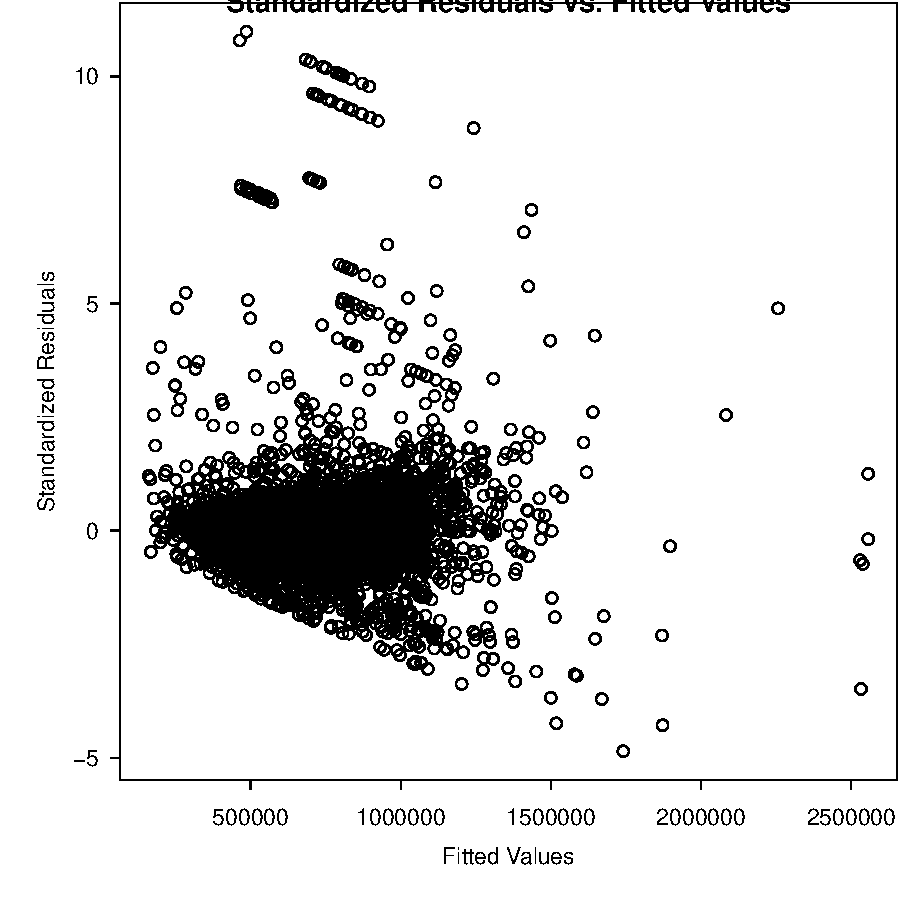
\includegraphics[width=.6\linewidth]{figure/assignment-8-2-Reppeto-Brian-Rnwauto-report-1} 

}


\begin{kframe}\begin{alltt}
\hlcom{## 13. Perform the necessary calculations to assess the assumption of no }
\hlcom{## multicollinearity and state if the condition is met or not.}

\hlstd{vif_values} \hlkwb{<-} \hlkwd{vif}\hlstd{(model_2)}


\hlkwd{print}\hlstd{(vif_values)}
\end{alltt}
\begin{verbatim}
##                 bedrooms          bath_full_count               year_built 
##                 1.580513                 1.585884                 1.339511 
## square_feet_total_living                sale_date 
##                 1.930920                 1.003585
\end{verbatim}
\begin{alltt}
\hlcom{# Overall, the VIF values for the predictor variables in the model are }
\hlcom{# relatively low, and none of them exceed a value of 5. This indicates that }
\hlcom{# there is no significant multicollinearity among the predictors in the model. }
\hlcom{# The VIF values being close to 1 for most variables suggest that the }
\hlcom{# predictors have little correlation with other predictors, supporting the }
\hlcom{# assumption of no multicollinearity in the model.}

\hlcom{## 14. Visually check the assumptions related to the residuals using the }
\hlcom{## plot() and hist() functions. Summarize what each graph is informing you of }
\hlcom{## and if any anomalies are present.}

\hlkwd{hist}\hlstd{(standardized_residuals,}
     \hlkwc{main} \hlstd{=} \hlstr{"Histogram of Standardized Residuals"}\hlstd{,}
     \hlkwc{xlab} \hlstd{=} \hlstr{"Standardized Residuals"}\hlstd{)}
\end{alltt}
\end{kframe}

{\centering 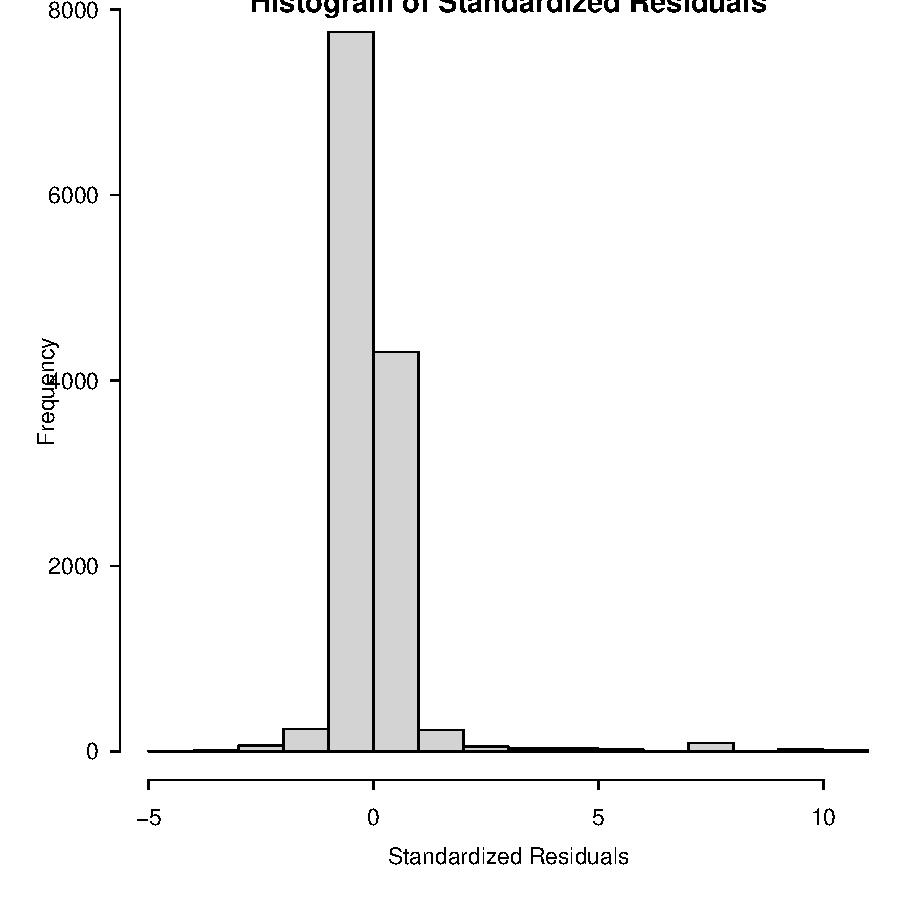
\includegraphics[width=.6\linewidth]{figure/assignment-8-2-Reppeto-Brian-Rnwauto-report-2} 

}


\begin{kframe}\begin{alltt}
\hlkwd{qqnorm}\hlstd{(standardized_residuals)}
\hlkwd{qqline}\hlstd{(standardized_residuals)}
\end{alltt}
\end{kframe}

{\centering 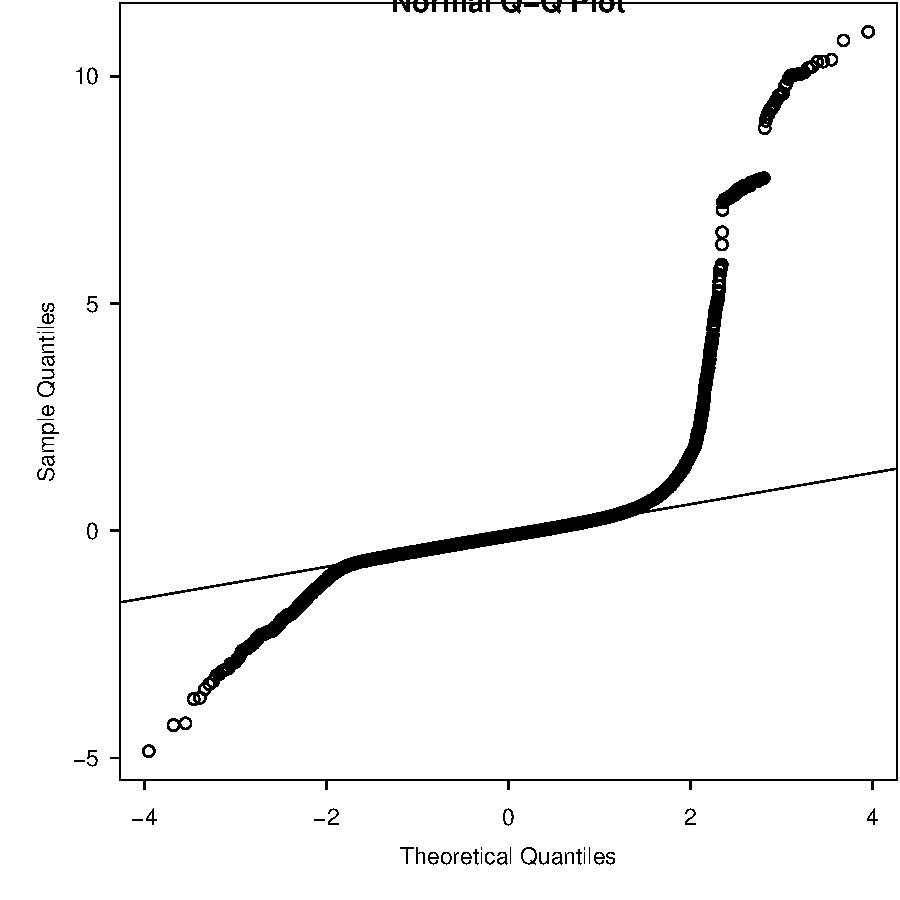
\includegraphics[width=.6\linewidth]{figure/assignment-8-2-Reppeto-Brian-Rnwauto-report-3} 

}


\begin{kframe}\begin{alltt}
\hlkwd{hist}\hlstd{(}\hlkwd{resid}\hlstd{(model_2),}
     \hlkwc{main} \hlstd{=} \hlstr{"Histogram of Residuals"}\hlstd{,}
     \hlkwc{xlab} \hlstd{=} \hlstr{"Residuals"}\hlstd{)}
\end{alltt}
\end{kframe}

{\centering 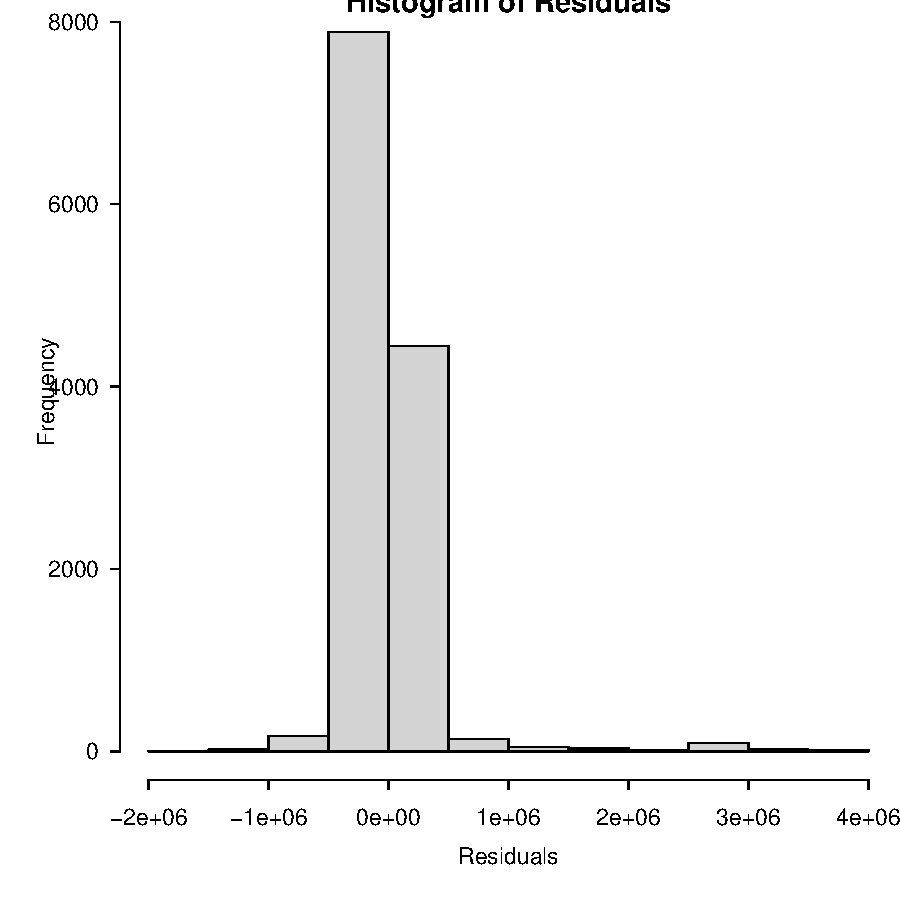
\includegraphics[width=.6\linewidth]{figure/assignment-8-2-Reppeto-Brian-Rnwauto-report-4} 

}


\begin{kframe}\begin{alltt}
\hlcom{## 15. Overall, is this regression model unbiased? If an unbiased regression }
\hlcom{## model, what does this tell us about the sample vs. the entire population }
\hlcom{## model?}

\hlcom{# Overall, the Model_2 appears to be unbiased. The unbiased regression model }
\hlcom{# provides estimates of the population parameters based on the sampled data.}
\hlcom{# However, the model validity depends on the quality of the sample and the }
\hlcom{# assumptions of the model. }
\end{alltt}
\end{kframe}
\end{knitrout}

The R session information (including the OS info, R version and all
packages used):

\begin{knitrout}
\definecolor{shadecolor}{rgb}{0.969, 0.969, 0.969}\color{fgcolor}\begin{kframe}
\begin{alltt}
\hlkwd{sessionInfo}\hlstd{()}
\end{alltt}
\begin{verbatim}
## R version 4.3.0 (2023-04-21)
## Platform: aarch64-apple-darwin20 (64-bit)
## Running under: macOS Ventura 13.4.1
## 
## Matrix products: default
## BLAS:   /System/Library/Frameworks/Accelerate.framework/Versions/A/Frameworks/vecLib.framework/Versions/A/libBLAS.dylib 
## LAPACK: /Library/Frameworks/R.framework/Versions/4.3-arm64/Resources/lib/libRlapack.dylib;  LAPACK version 3.11.0
## 
## locale:
## [1] en_US.UTF-8/en_US.UTF-8/en_US.UTF-8/C/en_US.UTF-8/en_US.UTF-8
## 
## time zone: America/New_York
## tzcode source: internal
## 
## attached base packages:
## [1] stats     graphics  grDevices utils     datasets  methods   base     
## 
## other attached packages:
##  [1] knitr_1.43       lm.beta_1.7-2    corrplot_0.92    lmtest_0.9-40    zoo_1.8-12      
##  [6] car_3.1-2        carData_3.0-5    conflicted_1.2.0 readxl_1.4.3     lubridate_1.9.2 
## [11] forcats_1.0.0    stringr_1.5.0    dplyr_1.1.2      purrr_1.0.1      readr_2.1.4     
## [16] tidyr_1.3.0      tibble_3.2.1     ggplot2_3.4.2    tidyverse_2.0.0 
## 
## loaded via a namespace (and not attached):
##  [1] utf8_1.2.3        generics_0.1.3    stringi_1.7.12    lattice_0.21-8   
##  [5] hms_1.1.3         magrittr_2.0.3    evaluate_0.21     grid_4.3.0       
##  [9] timechange_0.2.0  fastmap_1.1.1     cellranger_1.1.0  fansi_1.0.4      
## [13] scales_1.2.1      abind_1.4-5       cli_3.6.1         rlang_1.1.1      
## [17] munsell_0.5.0     withr_2.5.0       cachem_1.0.8      tools_4.3.0      
## [21] tzdb_0.4.0        memoise_2.0.1     colorspace_2.1-0  vctrs_0.6.3      
## [25] R6_2.5.1          lifecycle_1.0.3   pkgconfig_2.0.3   pillar_1.9.0     
## [29] gtable_0.3.3      glue_1.6.2        highr_0.10        xfun_0.39        
## [33] tidyselect_1.2.0  rstudioapi_0.15.0 xtable_1.8-4      compiler_4.3.0
\end{verbatim}
\begin{alltt}
\hlkwd{Sys.time}\hlstd{()}
\end{alltt}
\begin{verbatim}
## [1] "2023-07-30 16:13:57 EDT"
\end{verbatim}
\end{kframe}
\end{knitrout}


\end{document}
